\section{\projname Architecture}


\begin{figure}[t]
\vspace{-10pt}
\centering
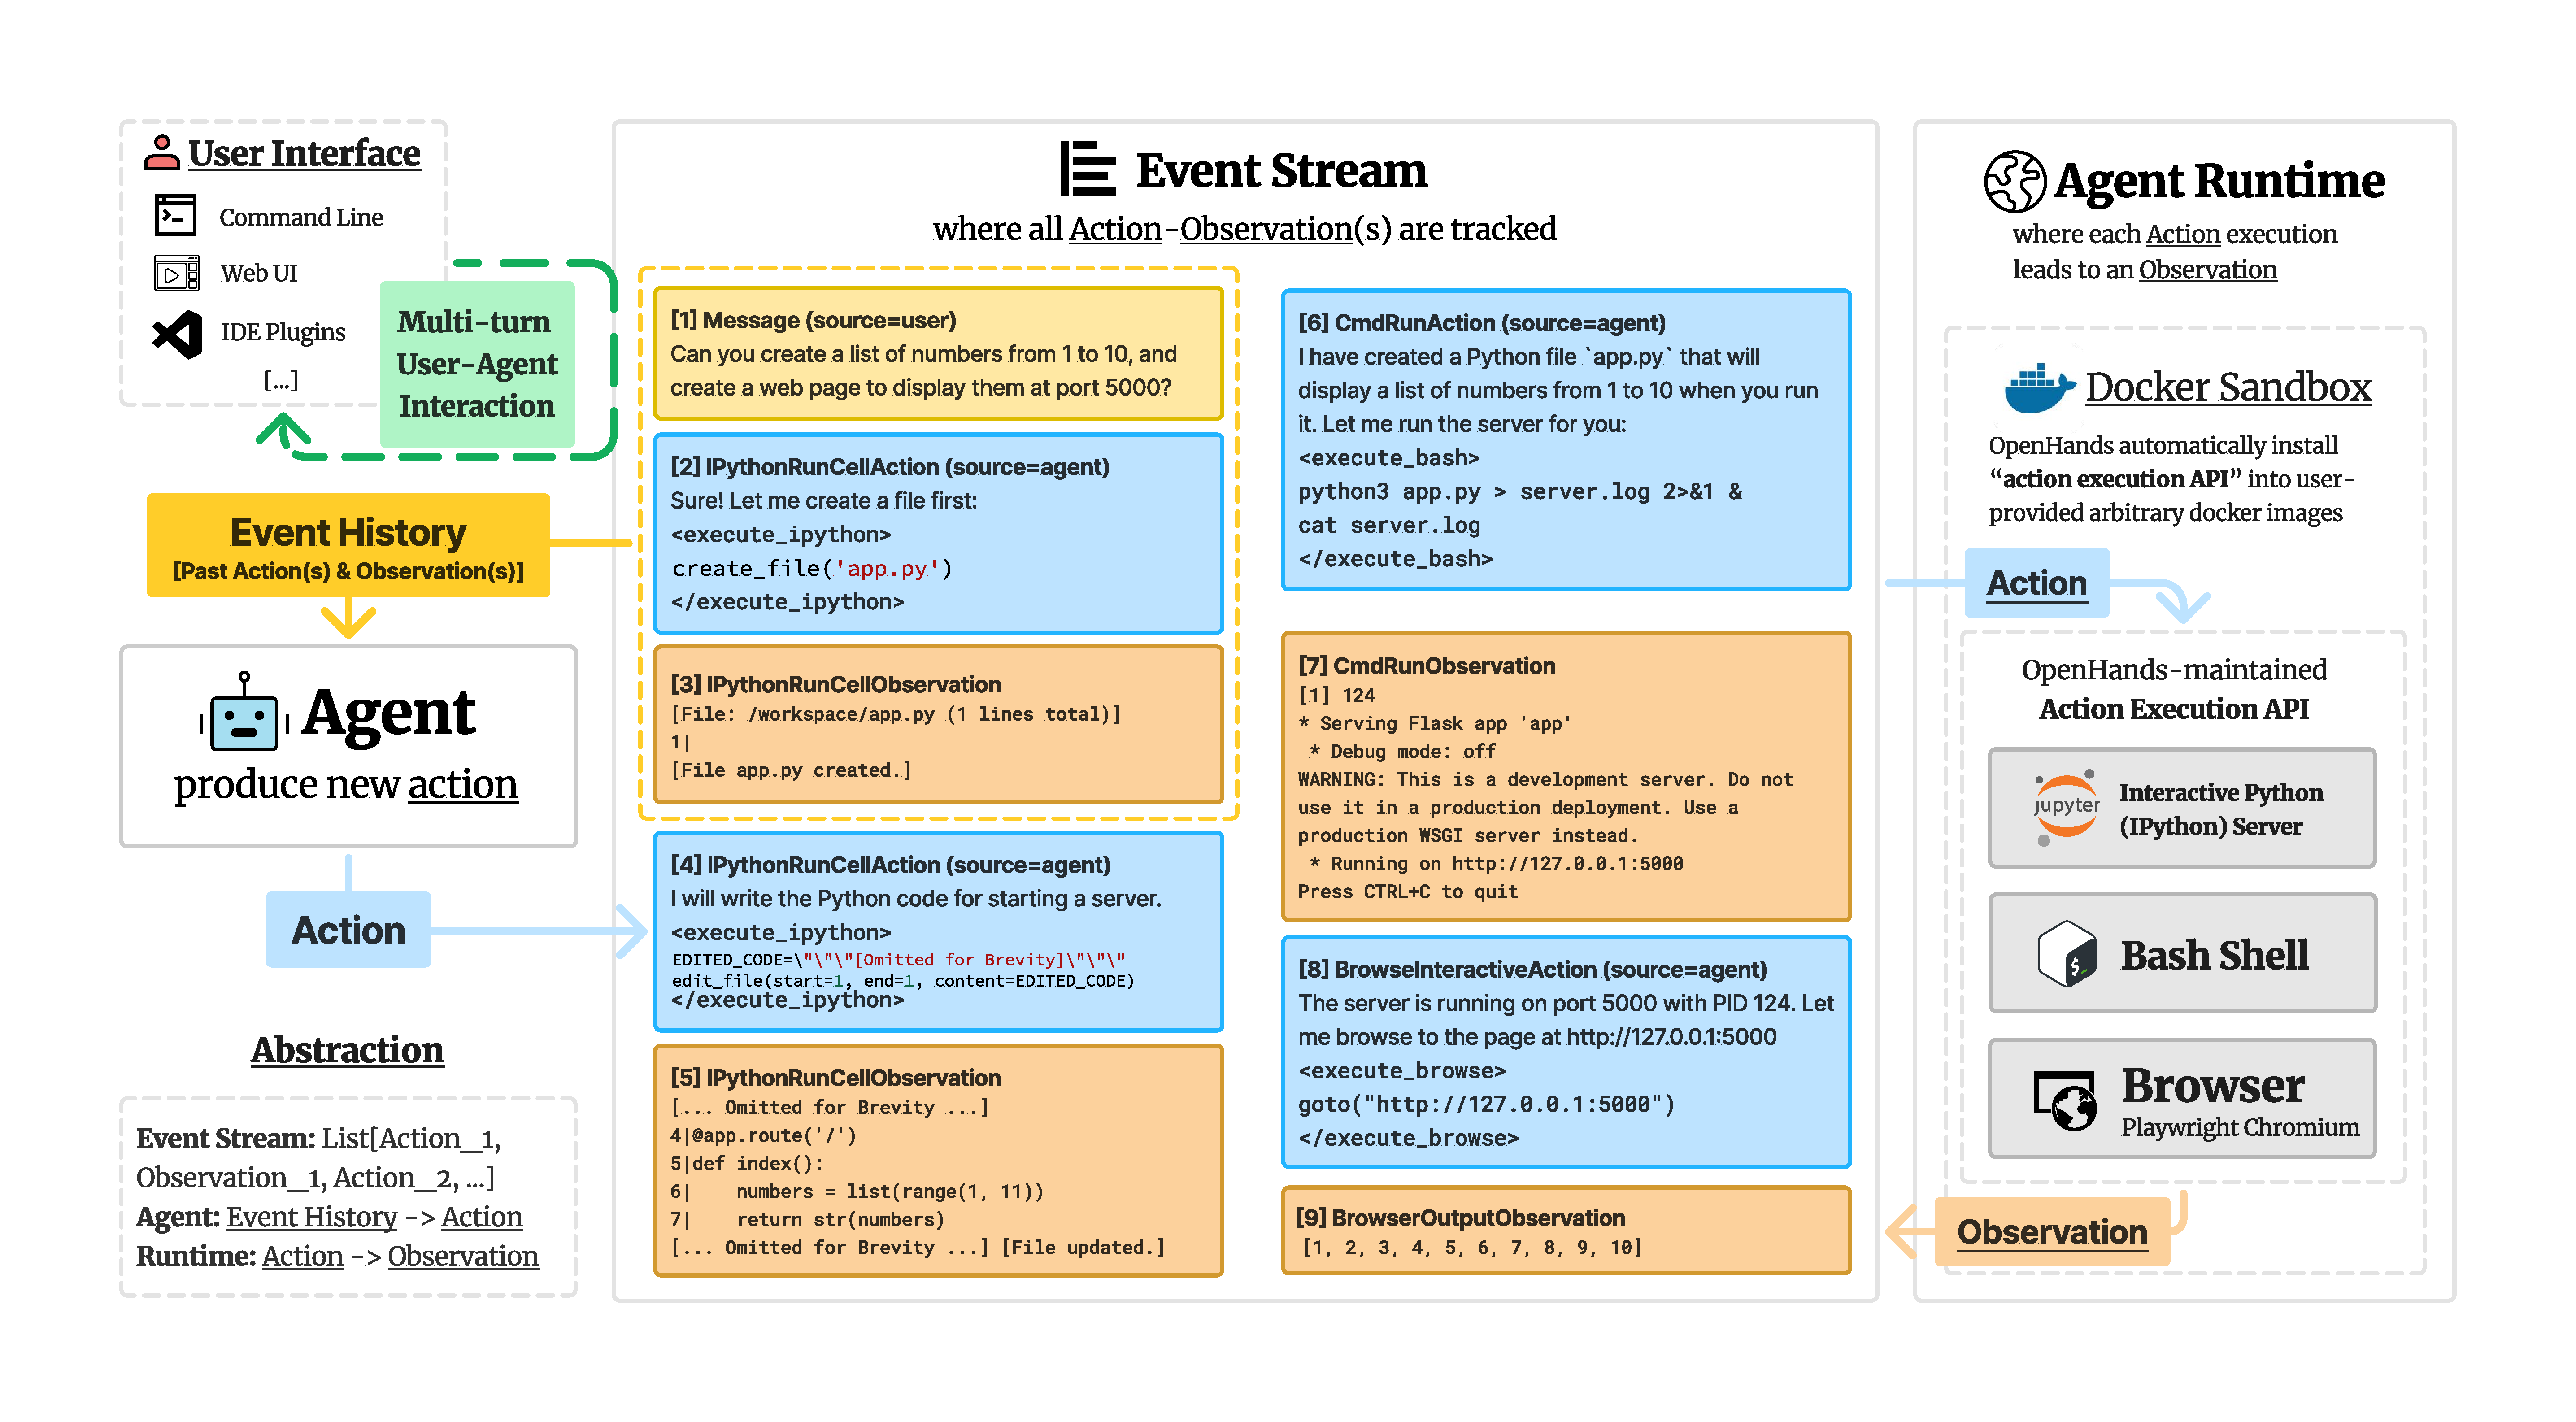
\includegraphics[clip, trim=4.5cm 4.5cm 4.5cm 4.5cm, width=\textwidth]{figs/oh_arch.pdf}
\caption{
\projname consists of 3 main components:
1) \textbf{Agent abstraction} where community can contribute different implementation of agents (\sref{sec:agent-abstraction}) into agenthub (\sref{sec:agenthub});
2) \textbf{Event stream} for tracking history of actions and observations; 
3) \textbf{Runtime} to execute all actions into observations (\sref{sec:agent-runtime}).
}
\vskip -0.15in
\label{fig:arch}
\end{figure}



We next describe using \projname in detail. In particular, we discuss 1) how to define and implement an agent (\sref{sec:agent-abstraction}), 2) how each action execution leads to an observation (\sref{sec:agent-runtime}), 3) how to reliably manage and extend commonly used skills for agents (\sref{sec:agent-skills}), and 4) how to compose multiple agents together for task solving (\sref{sec:agent-delegation}).
\fref{fig:arch} provides an overview.

\subsection{Agent Definition and Implementation}
\label{sec:agent-abstraction}


An \textbf{agent} can perceive the \textbf{state} of the environment (\eg, prior actions and observations) and produce an \textbf{action} for execution while solving a user-specified task.

\noindent \textbf{The State and Event Stream.} In \projname, the state is a data structure that encapsulates all relevant information for the agent's execution. A key component of this state is the \textbf{event stream}, which is a chronological collection of past actions and observations, including the agent's own actions and user interactions (\eg, instructions, feedback). In addition to the event stream, the state incorporates auxiliary information for agent's operation, such as the accumulative cost of LLM calls, metadata to track multi-agent delegation (\sref{sec:agent-delegation}), and other execution-related parameters. 


\noindent \textbf{Actions.} Inspired by CodeAct \citep{wang2024executable}, \projname connects an agent with the environment through a core set of general actions.
Actions \texttt{IPythonRunCellAction} and \texttt{CmdRunAction} enable the agent to execute \textit{arbitrary} Python code and bash commands inside the sandbox environment (\eg, a securely isolated Linux operating system).
\texttt{BrowserInteractiveAction} enables interaction with a web browser with a domain-specific language for browsing introduced by BrowserGym \citep{workarena2024}.
These actions were chosen to provide a comprehensive yet flexible set of primitives covering most tasks performed by human software engineers and analysts.
The action space based on programming languages (PL) is powerful and flexible enough to perform any task with tools in different forms (\eg, Python function, REST API, \etc) while being reliable and easy to maintain \citep{wang2024executable} .


\begin{wrapfigure}[21]{R}{0.6\textwidth}
\begin{minipage}{0.6\textwidth}
\vspace{-0.4cm}
\caption{Minimal example of implementing an agent in \projname.}
\vspace{-0.4cm}
\label{algo:agent-abstraction}
\begin{minted}[frame=lines,fontsize=\tiny]{python}
class MinimalAgent:
    def reset(self) -> None:
        self.system_message = "You are a helpful assistant ..."

    def step(self, state: State):
        messages: list[dict[str, str]] = [
            {'role': 'system', 'content': self.system_message}
        ]
        for prev_action, obs in state.history:
            action_message = get_action_message(prev_action)
            messages.append(action_message)
            obs_message = get_observation_message(obs)
            messages.append(obs_message)

        # use llm to generate response (e.g., thought, action)
        response = self.llm.do_completion(messages)

        # parse and execute action in the runtime
        action = self.parse_response(response)
        if self.is_finish_command(action):
            return AgentFinishAction()
        elif self.is_bash_command(action):
            return CmdRunAction(command=action.command)
        elif self.is_python_code(action):
            return IPythonRunCellAction(code=action.code)
        elif self.is_browser_action(action):
            return BrowseInteractiveAction(code=action.code)
        else:
            return MessageAction(content=action.message)
\end{minted}
\end{minipage}
\vspace{-2cm}
\end{wrapfigure}

This design is also compatible with existing tool-calling agents that require a list of pre-defined tools \citep{langchain2022}. That is, users can easily define tools using PL supported in primitive actions (\eg, write a Python function for calculator) and make those tools available to the agent through JSON-style function-calling experiences \citep{toolbench}.
Moreover, the framework's powerful PL-based primitives further make it possible for the agents to create tools by themselves (\eg, by generating Python functions, \citealt{craft}) when API to complete the task is unavailable.
Refer to \sref{sec:agent-skills} for how these core PL-based actions can be composed into a diverse set of tools.

\noindent \textbf{Observations.} Observations describe the environmental changes (\eg, execution result of prior actions, text messages from the human user \etc) that the agent observes. 

\noindent \textbf{Implement a New Agent.} 
The agent abstraction is designed to be simple yet powerful, allowing users to create and customize agents for various tasks easily.
The core of the agent abstraction lies in the \texttt{step} function, which takes the current state as input and generates an appropriate action based on the agent's logic. Simplified example code for the agent abstraction is illustrated in \fref{algo:agent-abstraction}.
By providing this abstraction, \projname allows the users to focus on defining desired agent behavior and logic without worrying about the low-level details of how actions are executed (\sref{sec:agent-runtime}).


\subsection{Agent Runtime: How Execution of Actions Results in Observations}
\label{sec:agent-runtime}


Agent Runtime provides a general environment that equips the agent with an action space comparable to that of human software developers, enabling \projname agents to tackle a wide range of software development and web-based tasks, including complex software development workflows, data analysis projects, web browsing tasks, and more.
It allows the agent to access a bash terminal to run code and command line tools, utilize a Jupyter notebook for writing and executing code on-the-fly, and interact with a web browser for web-based tasks (\eg, information seeking). 

\noindent \textbf{Docker Sandbox.} For each task session, \projname spins up a securely isolated docker container sandbox, where all the actions from the event stream are executed.
\projname connects to the sandbox through a REST API server running inside it (i.e., the \projname action execution API), executes arbitrary actions (e.g., bash command, python code) from the event stream, and returns the execution results as observations.
A configurable workspace directory containing files the user wants the agent to work on is mounted into that secure sandbox for \projname agents to access.

\noindent \textbf{\projname Action Execution API.} \projname maintains an API server that runs \textit{inside the docker sandbox} to listen for action execution requests from the event stream. The API server maintains:

\begin{itemize}[noitemsep,topsep=0pt,parsep=2pt,partopsep=0pt,leftmargin=18pt]
\item[(1)] A bash shell that connects with the operating system environment (specified by the docker image) for command execution.

\item[(2)] A Jupyter IPython server to handle interactive \emph{python} \citep{ipython} code execution requests and return the execution results back to the event stream.
\item[(3)] A Chromium browser based on \cite{playwright}. The provider provides a set of action primitives defined by BrowserGym \citep{browsergym, workarena2024}, such as navigation, clicking, typing, and scrolling. The full set of actions is detailed in \sref{sec:browsergym-actions}. 
After executing these actions, the browser runtime provides a rich set of observations about the current state of the browser, including HTML, DOM, accessibility tree~\citep{accessibilitytree}, screenshot, opened tabs, \etc.
\end{itemize}

\noindent \textbf{Arbitrary Docker Image Support.} \projname allows agents to run on arbitrary operating systems with different software environments by supporting runtime based on arbitrary docker images.
\projname implements a build mechanism that takes a user-provided arbitrary docker image and installs \projname action execution API into that image to allow for agent interactions.
We include a detailed description of \projname agent runtime in \sref{sec:runtime-details}.





\subsection{Agent Skills: The Extensible Agent-Computer Interface}
\label{sec:agent-skills}

SWE-Agent \citep{yang2024sweagent} highlights the importance of a carefully crafted Agent-Computer Interface (ACI, \ie, specialized tools for particular tasks) in successfully solving complex tasks.
However, creating, maintaining, and distributing a wide array of tools can be a daunting engineering challenge, especially when we want to make these tools available to different agent implementations (\sref{sec:agenthub}).
To tackle these, we build an \textbf{AgentSkills library}, a toolbox designed to enhance the capabilities of agents, offering utilities not readily available through basic \textit{bash} commands or \textit{python} code.

\textbf{Easy to create and extend tools.} AgentSkills is designed as a Python package consisting of different utility functions (\ie, tools) that are automatically imported into the Jupyter IPython environment (\sref{sec:agent-runtime}).
The ease of defining a Python function as a tool lowers the barrier for community members to contribute new tools to the library.
The generality of Python packages also allows different agent implementations to easily leverage these tools through one of our core action \texttt{IPythonRunCellAction} (\sref{sec:agent-abstraction}).



\textbf{Inclusion criteria and philosophy.} 
In the AgentSkills library, we do not aim to wrap every possible Python package and re-teach agents their usage (\eg, LLM already knows \texttt{pandas} library that can read CSV file, so we don't need to re-create a tool that teaches the agent to read the same file format).
We only add a new skill when: (1) it is not readily achievable for LLM to write code directly (\eg, edit code and replace certain lines), and/or (2) it involves calling an external model (\eg, calling a speech-to-text model, or model for code editing \citep{speculative_editing}).


\textbf{Currently supported skills.}
AgentSkills library includes file editing utilities adapted from SWE-Agent \citep{yang2024sweagent} and Aider \citep{aider} like \texttt{edit\_file}, which allows modifying an existing file from a specified line; scrolling functions \texttt{scroll\_up} and \texttt{scroll\_down} for viewing a different part of files.
It also contains tools that support reading multi-modal documents, like \texttt{parse\_image} and \texttt{parse\_pdf} for extracting information from images using vision-language models (\eg, GPT-4V) and reading text from PDFs, respectively.
A complete list of supported skills can be found in \sref{sec:supported-agentskills}.

\subsection{Agent Delegation: Cooperative Multi-agent Interaction}
\label{sec:agent-delegation}

\projname allows interactions between multiple agents as well. To this end, we use a special action type \texttt{AgentDelegateAction}, which enables an agent to delegate a specific subtask to another agent.
For example, the generalist CodeActAgent, with limited support for web-browsing, can use \texttt{AgentDelegateAction} to delegate web browsing tasks to the specialized BrowsingAgent to perform more complex browsing activity (\eg, navigate the web, click buttons, submit forms, \etc).


\begin{table}[!tbp]
\vskip -0.15in
\caption{
Comparison of different AI agent frameworks (\sref{sec:related_work}).
\textsc{Swe} refers to `software engineering'.
\textbf{Standardized tool library}: if framework contains reusable tools for different agent implementations (\sref{sec:agent-skills}); 
\textbf{Built-in sandbox \& code execution}: if it supports sandboxed execution of arbitrary agent-generated code;
\textbf{Built-in web browser}: if it provides agents access to a fully functioning web browser;
\textbf{Human-AI collaboration}: if it enables multi-turn human-AI collaboration (\eg, human can interrupt the agent during task execution and/or provide additional feedback and instructions);
\textbf{AgentHub}: if it hosts implementations of various agents (\sref{sec:agenthub});
\textbf{Evaluation Framework}: if it offers systematic evaluation of implemented agents on challenging benchmarks (\sref{sec:evaluation});
\textbf{Agent QC} (Quality Control): if the framework integrates tests (\sref{sec:integration-tests}) to ensure overall framework software quality.
}
\vspace{-0.2cm}
\label{tab:comparison}
\centering
\scriptsize
\begin{threeparttable}
\begin{adjustbox}{width=1\textwidth}
\begin{tabular}{ll|ccccccccc}
\toprule
\textbf{Framework} 
& \textbf{Domain} 
& \textbf{\makecell{Graphic\\ User Interface}}
& \textbf{\makecell{Standardized\\ Tool Library}}
& \textbf{\makecell{Built-in Sandbox\\ \& Code Execution}}
& \textbf{\makecell{Built-in Web\\ Browser}}
& \textbf{\makecell{Multi-agent\\ Collaboration}}
& \textbf{\makecell{Human-AI\\ Collaboration}} %
& \textbf{\makecell{AgentHub}} %
& \textbf{\makecell{Evaluation\\ Framework}}
& \textbf{\makecell{Agent\\ QC}} \\
\midrule

AutoGPT~\cite{gravitasauto} & General & \yes & \no & \no & \no & \no & \no & \yes & \no & \yes \\

LangChain~\citep{langchain2022} & General & \no & \yes & \no$^*$ & \no$^*$ & \no & \no & \yes & \no & \no \\
MetaGPT~\citep{hong2023metagpt} & General & \no & \yes & \no & \yes & \yes & \no & \yes & \no & \yes \\
AutoGen~\citep{wu2023autogen} & General & \no & \yes & \yes & \yes & \yes & \yes & \yes & \yes & \no \\
AutoAgents~\citep{chen2024autoagents} & General & \no & \no & \no & \no & \yes & \no & \no & \no & \no \\
Agents~\citep{zhou2023agents} & General & \no & \no & \no & \no & \yes & \yes & \no & \no & \no \\
Xagents~\citep{xagent2023} & General & \yes & \yes & \no & \yes & \yes & \no & \yes & \no & \no \\
OpenAgents~\citep{xie2023openagents} & General & \yes & \no & \yes & \yes & \no & \no & \yes & \no & \no \\
GPTSwarm~\citep{zhuge2024language} & General & \no & \yes & \no & \no & \yes & \yes & \no & \no & \no \\
\midrule
AutoCodeRover~\citep{zhang2024autocoderover} & SWE & \no & \no & \yes & \no & \no & \no & \no & \no & \no \\
SWE-Agent~\citep{yang2024sweagent} & SWE & \no & \no & \yes & \no & \no & \no & \no & \no & \no \\
\midrule
\textbf{\projname} & General & \yes & \yes & \yes & \yes & \yes & \yes & \yes & \yes & \yes \\
\bottomrule     
\end{tabular}
\end{adjustbox}
{
\tiny
\begin{tablenotes}
\item[*] No native support. Third-party commercial options are available.
\end{tablenotes}
}
\vskip -0.15in
\end{threeparttable}
\end{table}
